\documentclass[aspectratio=169]{beamer}

\usetheme{Madrid}
\usecolortheme{seahorse}
\usefonttheme{professionalfonts}

\usepackage{listings}
\usepackage{xcolor}
\usepackage{tikz}
\usepackage{booktabs}
\usepackage{hyperref}
\usepackage{textcomp}
\usepackage{microtype}

\definecolor{codebg}{HTML}{1E1E2E}
\definecolor{codegreen}{HTML}{A6E3A1}
\definecolor{codeblue}{HTML}{89DCEB}
\definecolor{codeyellow}{HTML}{F9E2AF}
\definecolor{codegray}{HTML}{6C7086}
\definecolor{codepurple}{HTML}{CBA6F7}
\definecolor{codeorange}{HTML}{FAB387}
\definecolor{codewhite}{HTML}{CDD6F4}
\definecolor{alertred}{HTML}{F38BA8}

\lstdefinestyle{clang}{
  backgroundcolor=\color{codebg},
  basicstyle=\ttfamily\footnotesize\color{codewhite},
  keywordstyle=\color{codepurple}\bfseries,
  commentstyle=\color{codegray}\itshape,
  stringstyle=\color{codegreen},
  numberstyle=\tiny\color{codegray},
  numbers=left, numbersep=6pt,
  breaklines=true, frame=single,
  rulecolor=\color{codeblue},
  language=C,
  tabsize=4
}

\title[MyOS Chapter 5]{\textbf{MyOS Chapter 5: Kernel Shell}}
\subtitle{From keyboard IRQ input to command-line control}
\author{MyOS Project}
\date{March 2026}
\institute{x86 Protected Mode Kernel Engineering}

\newcommand{\concept}[2]{%
  \begin{block}{#1}\smallskip #2\smallskip\end{block}\vspace{5pt}}

\newcommand{\warn}[1]{%
  \begin{alertblock}{Important}\smallskip #1\smallskip\end{alertblock}\vspace{5pt}}

\begin{document}

\begin{frame}
  \titlepage
\end{frame}

\begin{frame}{Stage goal ("Resume Gold" milestone)}
  \begin{itemize}
    \item Build an in-kernel interactive shell prompt: \texttt{MyOS>}
    \item Accept typed command lines through existing keyboard pipeline
    \item Implement commands: \texttt{help}, \texttt{clear}, \texttt{about}, \texttt{shutdown}
    \item Keep architecture stable (no direct heavy work inside IRQ handler)
  \end{itemize}
  \concept{Outcome}{
    MyOS moved from "display + input" to "interactive command execution".
  }
\end{frame}

\begin{frame}{How we achieved it (end-to-end path)}
\begin{center}
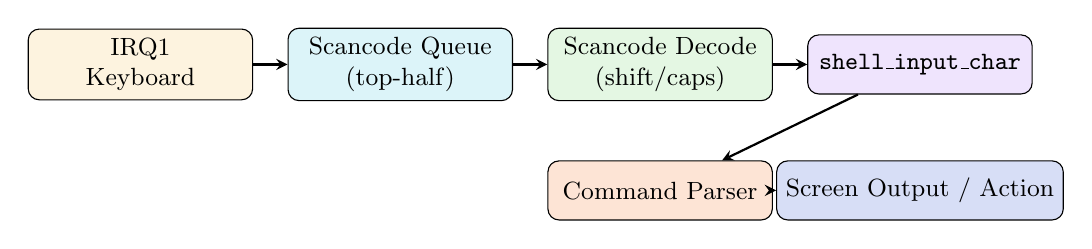
\begin{tikzpicture}[
  box/.style={rectangle,draw,rounded corners=4pt,
    minimum width=2.85cm,minimum height=0.75cm,
    align=center,font=\small},
  arr/.style={->,thick,>=stealth}]

  \node[box,fill=codeyellow!40] (irq) at (0,0) {IRQ1\\Keyboard};
  \node[box,fill=codeblue!30] (queue) at (3.3,0) {Scancode Queue\\(top-half)};
  \node[box,fill=codegreen!30] (decode) at (6.6,0) {Scancode Decode\\(shift/caps)};
  \node[box,fill=codepurple!30] (shell) at (9.9,0) {\texttt{shell\_input\_char}};

  \node[box,fill=codeorange!35] (exec) at (6.6,-1.6) {Command Parser};
  \node[box,fill=codewhite!80] (screen) at (9.9,-1.6) {Screen Output / Action};

  \draw[arr] (irq) -- (queue);
  \draw[arr] (queue) -- (decode);
  \draw[arr] (decode) -- (shell);
  \draw[arr] (shell) -- (exec);
  \draw[arr] (exec) -- (screen);
\end{tikzpicture}
\end{center}
\end{frame}

\begin{frame}{Pre-existing modules we changed}
  \small
  \begin{tabular}{@{}p{2.4cm}p{3.7cm}p{5.7cm}@{}}
    \toprule
    \textbf{Module} & \textbf{Before} & \textbf{Change for shell stage} \\
    \midrule
    \texttt{kernel.c} & Boot banner + IRQ enable + loop & Calls \texttt{shell\_init()} after \texttt{sti}; keeps polling \texttt{keyboard\_process\_pending()}. \\
    \texttt{keyboard.c} & Decoded keys printed directly to screen & Decoded chars now routed to \texttt{shell\_input\_char(c)}; queue logic retained. \\
    \texttt{Makefile} & Built core kernel objects & Added \texttt{shell.c} compilation and link object \texttt{shell.o}. \\
    \texttt{screen.c} & Text rendering + cursor + scrollback & Reused unchanged as shell output backend. \\
    \bottomrule
  \end{tabular}
\end{frame}

\begin{frame}[fragile]{New module: \texttt{shell.c}}
\begin{lstlisting}[style=clang]
void shell_init() {
    input_len = 0;
    print_prompt();
}

void shell_input_char(char c) {
    if (c == '\b') { ... }      // edit line buffer
    if (c == '\n') { ... }      // execute command
    if (printable) { ... }       // append + echo
}
\end{lstlisting}
\textbf{Design notes:}
\begin{itemize}
  \item Fixed-size input buffer: \texttt{SHELL\_MAX\_INPUT = 64}
  \item Prompt colorized via \texttt{set\_color(0x0E)} then restored
  \item Unknown commands return help hint (friendly UX)
\end{itemize}
\end{frame}

\begin{frame}[fragile]{Command execution logic}
\begin{lstlisting}[style=clang]
static void execute_command(const char* cmd) {
    if (str_equals(cmd, "help")) { ... }
    if (str_equals(cmd, "clear")) { clear_screen(); return; }
    if (str_equals(cmd, "about")) { ... }
    if (str_equals(cmd, "shutdown")) {
        outw(0x604, 0x2000);
        cli; hlt-loop;
    }
    print("Unknown command ...");
}
\end{lstlisting}
\concept{Reasoning}{
  Simple string matching is enough for early kernel shell stage; no dynamic memory, no parser complexity.
}
\end{frame}

\begin{frame}{Command-by-command behavior}
  \begin{itemize}
    \item \texttt{help}: prints all available commands and short descriptions
    \item \texttt{clear}: clears VGA terminal and returns to fresh prompt
    \item \texttt{about}: prints project identity/motivation message
    \item \texttt{shutdown}: sends ACPI poweroff signal through QEMU-compatible port
  \end{itemize}
  \warn{If \texttt{shutdown} does not power off on a real machine, that is expected. It is emulator/platform-dependent.}
\end{frame}

\begin{frame}[fragile]{Integration in \texttt{kernel.c}}
\begin{lstlisting}[style=clang]
print("Enabling interrupts...\n");
__asm__ volatile("sti");
print("Interrupts enabled. Keyboard ready.\n");
shell_init();

while (1) {
    __asm__ volatile("hlt");
    keyboard_process_pending();
}
\end{lstlisting}
\textbf{Why this placement?}
\begin{itemize}
  \item Prompt appears only after interrupt path is live
  \item Main loop remains low-power with \texttt{hlt}
  \item Input processing is deterministic and serialized
\end{itemize}
\end{frame}

\begin{frame}[fragile]{Integration in \texttt{keyboard.c}}
\begin{lstlisting}[style=clang]
if (scancode < 128) {
    ... // map to char with shift/caps logic
}

if (c != 0) {
    shell_input_char(c);
}
\end{lstlisting}
\concept{Architectural benefit}{
  Keyboard keeps doing hardware decoding; shell owns command semantics.
  This separation avoids mixing device-driver code with command policy.
}
\end{frame}

\begin{frame}[fragile]{Build system update (Makefile)}
\begin{lstlisting}[style=clang]
SHELL_C  := kernel/shell.c

$(BUILD)/shell.o: $(SHELL_C) | $(BUILD)
    $(CC) $(CFLAGS) -c $< -o $@

$(BUILD)/kernel.bin: ... $(BUILD)/shell.o
\end{lstlisting}
\textbf{Result:}
\begin{itemize}
  \item Shell is now a first-class kernel module
  \item No manual linker edits needed outside Makefile object list
\end{itemize}
\end{frame}

\begin{frame}{Keyword glossary (core shell terms)}
  \small
  \begin{tabular}{@{}p{2.8cm}p{9.2cm}@{}}
    \toprule
    \textbf{Keyword} & \textbf{Meaning in this stage} \\
    \midrule
    \texttt{Prompt} & Text prefix indicating shell is ready (\texttt{MyOS>}). \\
    \texttt{REPL-like loop} & Read input, evaluate command, print result, show prompt again. \\
    \texttt{Input buffer} & Temporary line storage before pressing Enter. \\
    \texttt{Backspace} & Edits both on-screen text and input buffer state. \\
    \texttt{Command parser} & Maps string command to kernel action. \\
    \texttt{Dispatch} & Selecting which command handler runs. \\
    \texttt{Top-half} & IRQ context: minimal and fast (queue scancode). \\
    \texttt{Bottom-half} & Non-IRQ context: decode/process/execute command. \\
    \bottomrule
  \end{tabular}
\end{frame}

\begin{frame}{Keyword glossary (hardware/control terms)}
  \small
  \begin{tabular}{@{}p{2.8cm}p{9.2cm}@{}}
    \toprule
    \textbf{Keyword} & \textbf{Meaning in this stage} \\
    \midrule
    \texttt{IRQ1} & Keyboard interrupt source line. \\
    \texttt{EOI} & End-of-interrupt command sent to PIC after handling IRQ. \\
    \texttt{inb(0x60)} & Read keyboard controller scancode byte. \\
    \texttt{hlt} & CPU sleep until next interrupt (efficient idle loop). \\
    \texttt{sti} & Enable maskable interrupts globally. \\
    \texttt{outw(0x604, 0x2000)} & QEMU/ACPI-style shutdown request port write. \\
    \texttt{freestanding} & Kernel build mode without host standard library/runtime. \\
    \bottomrule
  \end{tabular}
\end{frame}

\begin{frame}{Verification checklist for Chapter 5}
  \begin{enumerate}
    \item Boot and verify prompt \texttt{MyOS>} appears
    \item Type \texttt{help} and confirm command list
    \item Type unknown command and verify fallback message
    \item Type \texttt{clear} and verify screen resets + prompt returns
    \item Type \texttt{about} and verify project message
    \item Type \texttt{shutdown} and verify emulator poweroff/stop behavior
  \end{enumerate}
\end{frame}

\begin{frame}{What this unlocks next}
  \vspace{8pt}
  \begin{center}
    \Large \textbf{Chapter 5 turns MyOS into an interactive kernel environment.}
  \end{center}
\end{frame}

\end{document}
